\section{Trådløs kommunikation gennem Bluetooth Low Energy}
\textit{I dette afsnit gennemgår design, implementering og test af systemets trådløse kommunikation mellem de to benyttede MCUer.}

\subsection{Design}
Systemet vil involvere to MCUer, henholdsvis en GAP central og en GAP peripheral. Begge enheder vil have påført et BLE modul, således dataoverførslen mellem enhederne vil foregå gennem brug af BLE. Denne dataoverførsel mellem MCUerne er illustreret som pseudokode på \figref{fig:blue_pseudo}. 

\begin{figure}[H]
	\centering
	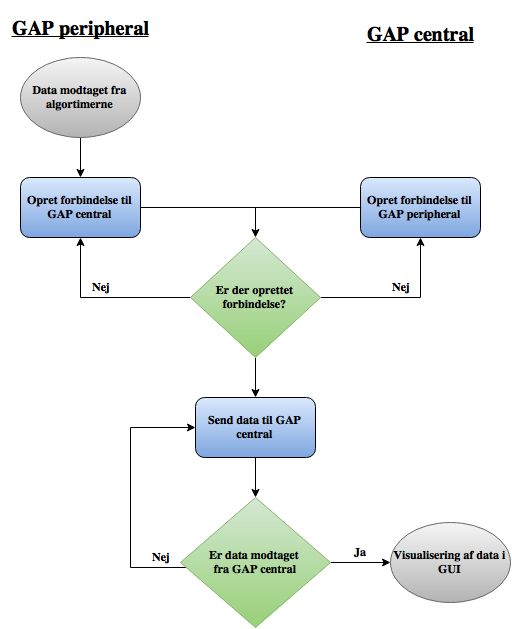
\includegraphics[scale=0.5]{figures/cDesign/blue_pseudo.png}
	\caption{Illustration af den trådløse kommunikation og dataoverførsel mellem GAP central og GAP peripheral. Indledningsvis forsøges det at oprette forbindelse mellem enhederne, hvorefter dataoverførslen finder sted. Ved fuldendt dataoverførsel bliver BLE modulet for de to enheder slukket/sat i dvale.}
	\label{fig:blue_pseudo}
\end{figure}
Ovenstående pseudokode er bestemmende for  for hvorvidt en MCU vil fungere som GAP central eller peripheral i et kredsløb. Den enhed som initialiseres til GAP central skal modtage data fra den anden enhed. Ydermere skal GAP central overføre denne data til en computer gennem en USB port, således visualisering i et GUI er mulig. \newline
Førend en dataoverførsel er mulig, er det nødvendigt at der er skabt en forbindelse mellem de to enheder, hvilket ligeledes fremgår af \figref{fig:blue_pseudo}. Hvis ikke det lykkes at oprette forbindelse, gentages denne procedure. Når der er etableret forbindelse mellem enhederne overføres dataene, som modtages fra algoritmerne fra PSoC 4200M. Ydermere vil systemet ikke fortsætte til næste element i pseudokoden, medmindre dataoverførslen har været succesfuld.  

\subsection{Implementering}
GAP peripheral er den MCU som er ansvarlig for dataopsamling, signalbehandling og afsendelse af data til GAP central. GAP peripheral vil dermed benytte et samarbejde mellem PSoC 4200M og EZ-BLE. Konfigureringen af henholdsvis GAP central og GAP peripheral udføres i PSoC Creator, hvor ’Topdesign’ af EZ-BLE modulerne er afgørende for deres rolle i kredsen. \newline
PSoc 4200M på GAP peripheral vil blive konfigureret således dataoverførslen vil blive ført mod EZ-BLE. Denne konfigurering udføres ved at initialisere de pågældende pins for PSoC 4200M og EZ-BLE i pindesign i PSoC Creator. Port P3[0] bliver benyttet til UART:rx og port P3[1] til UART:tx. Ydermere konfigureres EZ-BLE modulet til at benytte P1[4] til UART:rx og port P1[5] til UART:tx. Disse konfigureringer sikrer at der forekommer en dataoverførsel fra PSoC 4200M og videre til EZ-BLE, hvorfra dataene kan sendes til GAP central. \citep{Semiconductor20164200M} \newline
GAP central skal konfigureres, således denne kan modtage data og herefter overføre dette til en computer gennem USB porten. For at sikre disse handlinger, benyttes samme pins til UART mellem EZ-BLE og PSoC 4200M. Ydermere benyttes port P7[0] til UART:rx og port P7[1] til UART:tx. Dermed er det muligt at overføre datene fra PSoC LP5 til en computer. 

Det fremgår af \figref{fig:blue_pseudo}, at BLE modulerne skal sættes slukkes når dataoverførslen er fuldendt. Derfor vil C kodning af BLE modulerne medvirke til, at denne handling er mulig. \textbf{DER SKAL NOK SKRIVER MERE HERTIL NÅR VI VED HVORDAN VI BENYTTER POWERMODES.}

\subsection{Test}
Den trådløse kommunikation testes for at undersøge kvaliteten af forbindelsen mellem GAP peripheral og GAP central. GAP peripheral bliver sat til at videresende datapakker, hvoraf GAP central  vil modtage disse datapakker, hvis dataoverførslen er nøjagtig vil der ikke mangle nogle pakker. Dette vil blive illustreret igennem MATLAB, hvoraf en nøjagtig overførsel vil medføre en fuldstændig lineær kurve. Hvis datapakker er gået tabt vil illustrationen af antal modtagne pakker varierer fra antal sendte pakker, med stor hældning og den kurven vil ikke være lineær. Denne test udføres med forskellig afstand mellem GAP peripheral og GAP central, hvoraf den maksimale afstand for succesfuld dataoverførsel vil komme til udtryk. \\
Datapakkerne i denne test sendes fire gange i sekundet, og resultaterne bliver opsamlet igennem 30 sekunder. Der skabes forbindelse mellem GAP peripheral og GAP central og antallet af modtagne datapakker optages igennem RealTerm.
\begin{table}[H]
	\centering
	\begin{tabular}{ccccccccc}
		\rowcolor[HTML]{C0C0C0} 
		Afstand {[}m{]} & 0,5 & 1 & 1,5 & 2 & 2,5 & 3 & 3,5 & 4  \\
		Antal tabte datapakke & 0 & 0 & 0 & 0 & 0 & 0 & 0 & Trådløs forbindelse tabt 
	\end{tabular}
	\caption{I tabellen ses sammenhængen mellem antal tabte datapakker og afstanden mellem GAP peripheral og GAP central.}
	\label{test:ble_overforsel}
\end{table} \vspace{-.5cm}
Testresultaterne viste at ved trådløs overførsel imellem GAP peripheral og GAP central skulle afstanden herimellem være over 3,5 meter, før den trådløse forbindelse gik tabt.
\begin{figure}[H]
	\centering
	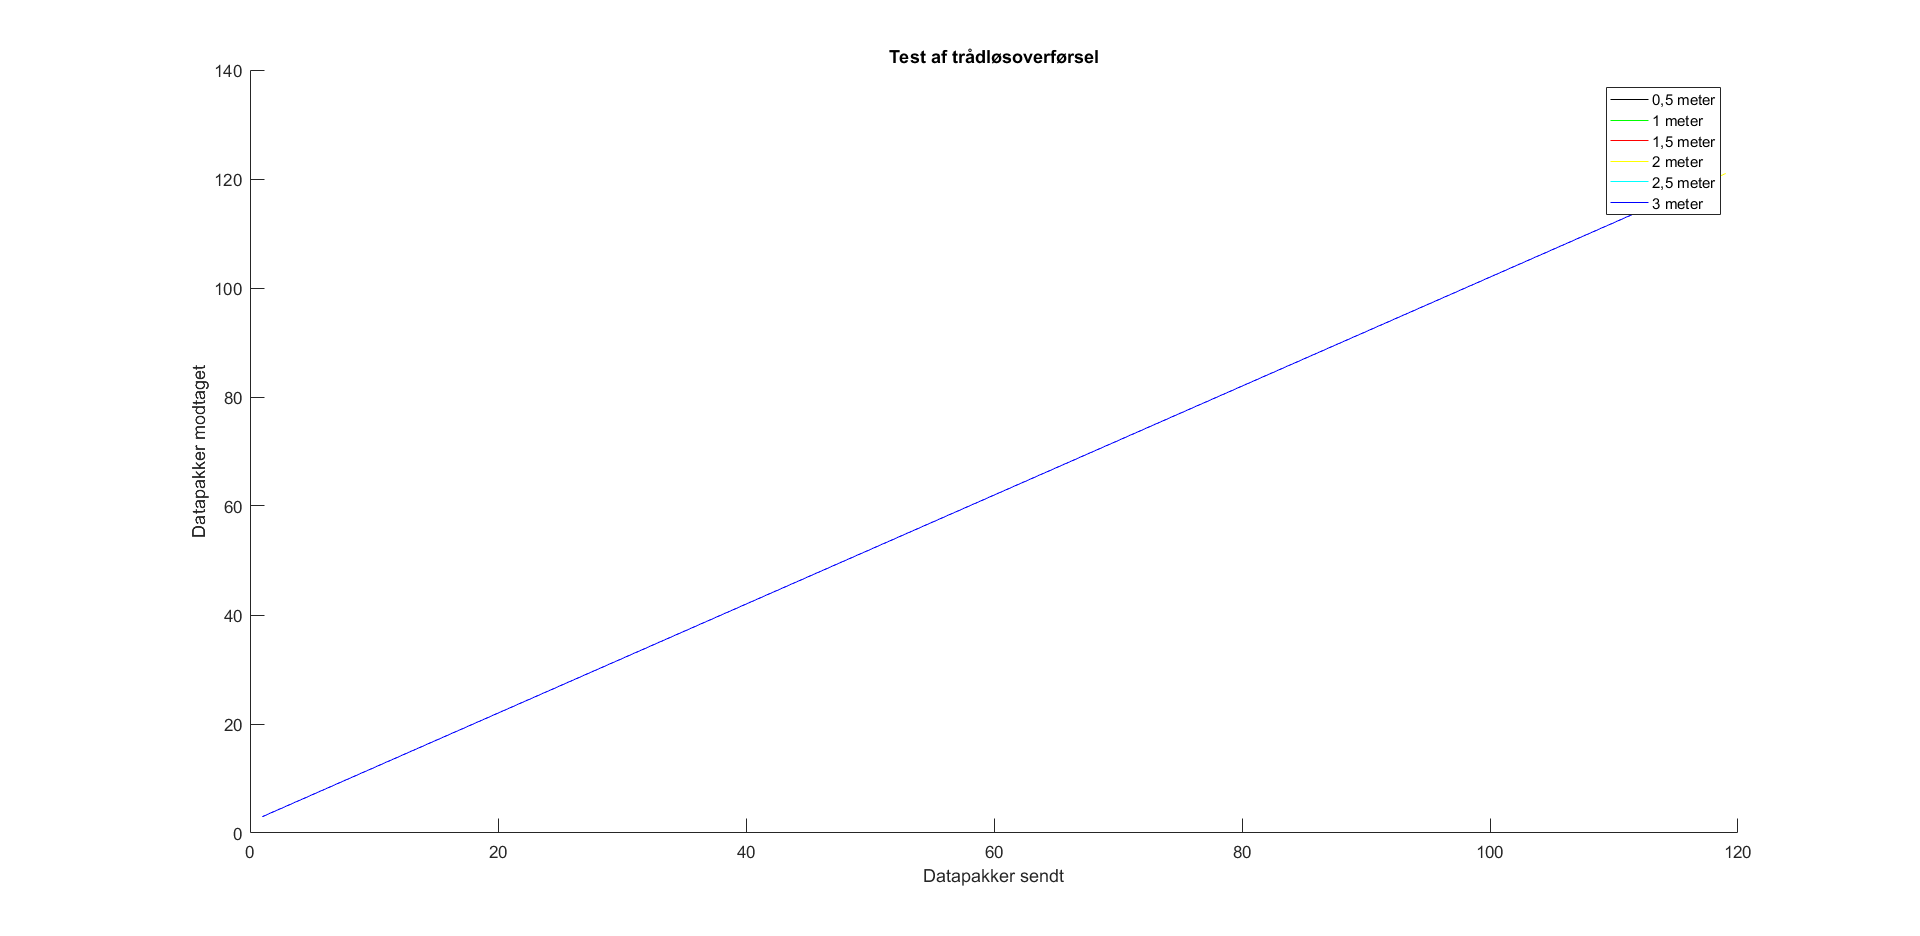
\includegraphics[scale=0.3]{figures/cDesign/test_ble.png}
	\caption{På figuren ses et grafisk plot af forholdet mellem antal sendte og antal modtagne datapakker. }
	\label{fig:test_ble}
\end{figure}
Resultatet af at alle datapakker blev modtaget, så forekommer der ingen udsalg på den grafiske illustration, som ses på \figref{fig:test_ble}. På grafen er den eneste kurve der kommer til udtryk den blå kurve tilhørende resultatet af en afstand på 3,5 meter. Dette er resultatet af at ingen af de foregående afstande har mistet nogle datapakker, og kurverne befinder sig præcist oveni hinanden. Hvis afstanden mellem GAP peripheral og GAP central overskrider 3,5 meter, så brydes forbindelsen heraf og datapakkerne bliver ikke sendt. \\
Den trådløse kommunikation mellem systemets enheder overholder kravet vedrørende afsendelse og modtagelse af korrekt data inden for 3 meters afstand. Kravet vedrørende tab af data heraf overholdes ligeledes, da datapakker først går tabt ved 4 meters afstand. 
